\documentclass[12pt,]{article}
%\usepackage{lmodern}  Melissa removed to deal with font rendering issue
\usepackage{amssymb,amsmath}
\usepackage{ifxetex,ifluatex}
\usepackage{fixltx2e} % provides \textsubscript

%Melissa removed the following section to deal with font rendering issue
%\ifnum 0\ifxetex 1\fi\ifluatex 1\fi=0 % if pdftex
%  \usepackage[T1]{fontenc}
%  \usepackage[utf8]{inputenc}
%%\else % if luatex or xelatex
%  \ifxetex
%    \usepackage{mathspec}
%  \else
%    \usepackage{fontspec}
%  \fi
%  \defaultfontfeatures{Ligatures=TeX,Scale=MatchLowercase}
%  \newcommand{\euro}{€}
%%%%%%\fi

% use upquote if available, for straight quotes in verbatim environments
\IfFileExists{upquote.sty}{\usepackage{upquote}}{}
% use microtype if available
\IfFileExists{microtype.sty}{%
\usepackage{microtype}
\UseMicrotypeSet[protrusion]{basicmath} % disable protrusion for tt fonts
}{}
\usepackage[margin=1in]{geometry}
\usepackage{hyperref}
\PassOptionsToPackage{usenames,dvipsnames}{color} % color is loaded by hyperref
\hypersetup{unicode=true,
            pdftitle={Status of A Fish (Beringraja binoculata) Off the U.S. Pacific Coast in 2017},
            pdfborder={0 0 0},
            breaklinks=true}
\urlstyle{same}  % don't use monospace font for urls
\setlength{\parindent}{0pt}
\setlength{\parskip}{6pt plus 2pt minus 1pt}
\setlength{\emergencystretch}{3em}  % prevent overfull lines
\providecommand{\tightlist}{%
  \setlength{\itemsep}{0pt}\setlength{\parskip}{0pt}}
\setcounter{secnumdepth}{5}

%%% Use protect on footnotes to avoid problems with footnotes in titles
\let\rmarkdownfootnote\footnote%
\def\footnote{\protect\rmarkdownfootnote}

%%% Change title format to be more compact
\usepackage{titling}

% Create subtitle command for use in maketitle
\newcommand{\subtitle}[1]{
  \posttitle{
    \begin{center}\large#1\end{center}
    }
}

\setlength{\droptitle}{-2em}
  \title{Status of A Fish (\emph{Beringraja binoculata}) Off the U.S. Pacific
Coast in 2017}
  \pretitle{\vspace{\droptitle}\centering\huge}
  \posttitle{\par}
  \author{}
  \preauthor{}\postauthor{}
  \date{}
  \predate{}\postdate{}


% This file contains all of the LaTeX packages you may need to compile the document
% Documentation for each package can be found onlines
\usepackage{tabularx}                                             % table environment providing flexibility
\usepackage{caption}                                              % for creating captions  
\usepackage{longtable}                                            % allows tables to span multiple pages
\usepackage{rotating}                                             % allows for sideways tables
\usepackage{float}                                                % floating environments; may not need in rmarkdown
\usepackage{placeins}                                             % keeps floats from moving
\usepackage{indentfirst}                                          % indents first paragraph of a section
\usepackage{mdwtab}                                               % continued float multi-page figure
\usepackage{enumerate}                                            % create lists
\usepackage{hyperref}                                             % highlight cross references
\hypersetup{colorlinks=true, urlcolor=blue, linktoc=page, linkcolor=blue, citecolor=blue} %define referencing colors
%\usepackage{makebox}                                             % make boxes around text
\usepackage[usenames,dvipsnames]{xcolor}                          % color name options
%\usepackage[space]{grffile}                                      % spaces in file name path
\usepackage{soul}                                                 % highlight text
\usepackage{enumitem}                                             % numbered lists
\usepackage{lineno}                                               % Line numbers; comment out for final
\usepackage{upquote}                                              % produce grave accent in latex
\usepackage{verbatim}                                             % produces verbatim results
\usepackage{fancyvrb}                                             % verbatim in a box
%\usepackage{draftwatermark}                                      % places Draft watermark in background; comment out for final
\usepackage{textcomp}                                             % fixes error with packages interfering
\usepackage{lscape}                                               % rotate pages - to allow for landscape longtables
%\pdfinterwordspaceon                                             % fix loss of inter word spacing
\usepackage{cmap}                                                 % fix mapping characters to unicode
\RequirePackage[linewidth = 1]{pdfcomment}                        % pdf comments
\RequirePackage[l2tabu, orthodox]{nag}                            % checks packages related to the accessibility?
\usepackage[inline]{showlabels}                                   % show table and figure labels; comment out for final
%\RequirePackage[tagged]{accessibilityMeta}


\linenumbers                                                      % specify use of line numbers


\definecolor{light-gray}{gray}{.85}                               % define light-gray as a color
%\usepackage[tagged]{accessibility-meta}

 
%\showlabels[\color{mred}]{label}

% Redefines (sub)paragraphs to behave more like sections
\ifx\paragraph\undefined\else
\let\oldparagraph\paragraph
\renewcommand{\paragraph}[1]{\oldparagraph{#1}\mbox{}}
\fi
\ifx\subparagraph\undefined\else
\let\oldsubparagraph\subparagraph
\renewcommand{\subparagraph}[1]{\oldsubparagraph{#1}\mbox{}}
\fi

\begin{document}
\maketitle


\begin{center}
\thispagestyle{empty}


\vspace{.5cm}

%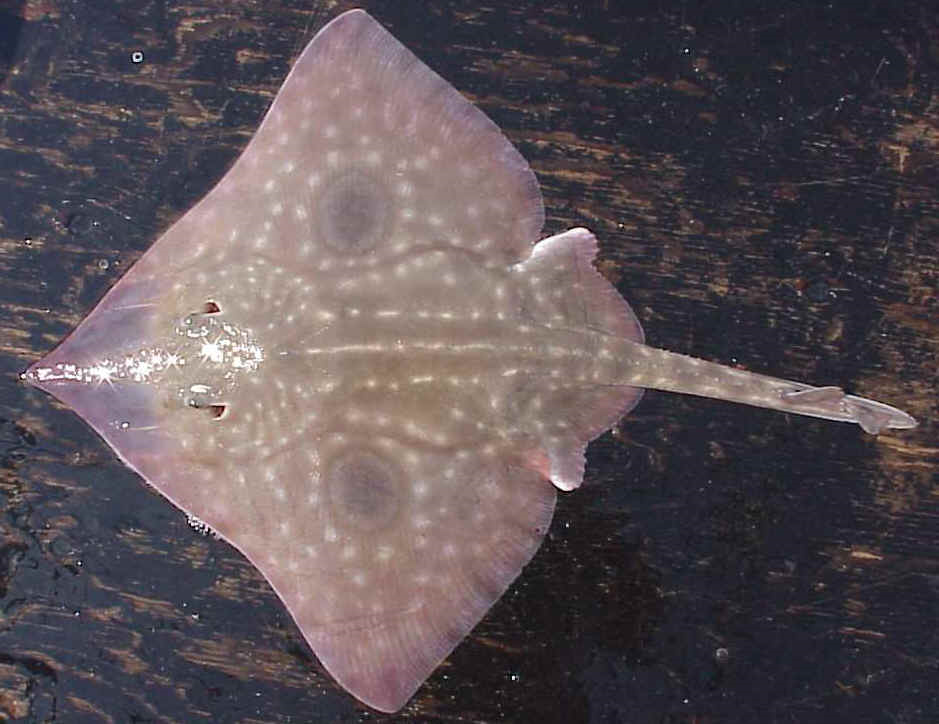
\includegraphics{cover_photo}~\\[1cm]
\pdftooltip{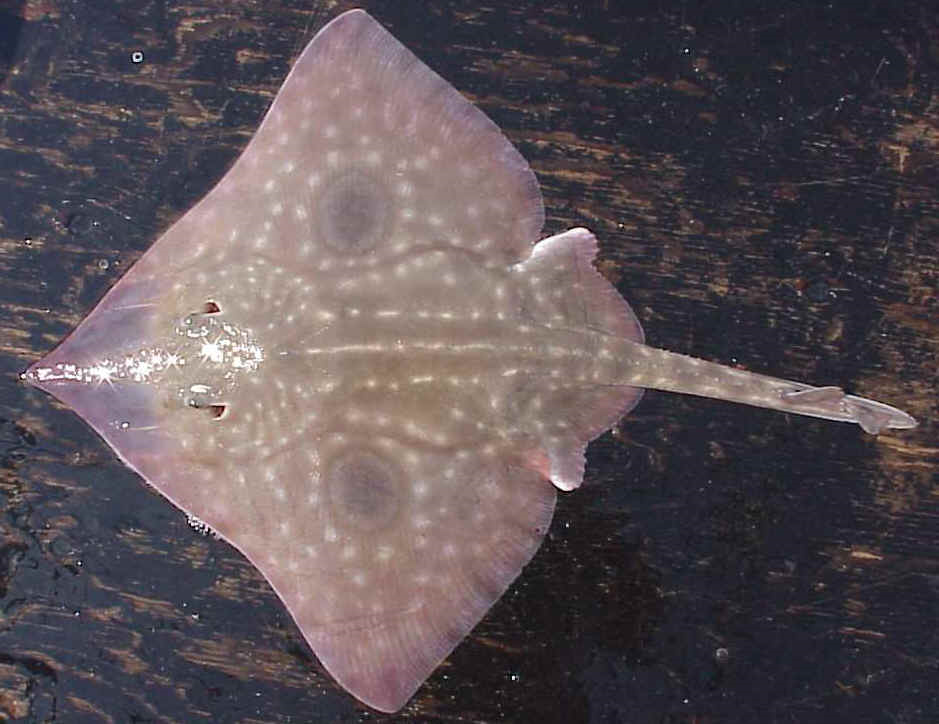
\includegraphics{cover_photo}}{This is a fish.}



Author No. 1\textsuperscript{1}\\
Author No. 2\textsuperscript{2}\\
Author No. 3\textsuperscript{3}\\

\vspace{.5cm}

\small
\textsuperscript{1}Southwest Fisheries Science Center, U.S. Department of Commerce, National Oceanic and Atmospheric Administration, National Marine Fisheries Service, 110 Shaffer Road, Santa Cruz, California 95060\\

\vspace{.3cm}

\textsuperscript{2}Northwest Fisheries Science Center, U.S. Department of Commerce, National Oceanic and Atmospheric Administration, National Marine Fisheries Service, 2725 Montlake Boulevard East, Seattle, Washington 98112\\

\vspace{.3cm}

\textsuperscript{3}Washington Department of Fish and Wildlife, 600 Capitol Way North, Olympia, Washington 98501\\


\vspace{.5cm}

\vfill
DRAFT SAFE\\
Disclaimer: This information is distributed solely for the purpose of pre-dissemination
peer review under applicable information quality guidelines. It has not been formally
disseminated by NOAA Fisheries. It does not represent and should not be construed to
represent any agency determination or policy. 

\vspace{.3cm}
%Bottom of the page
%{\large \today}


\newpage{\thispagestyle{empty}}


\begin{flushleft}
This report may be cited as:

ex. Monk, M. H. ,He, X., and Budrick, J. 2017. Status of the California Scorpionfish (\emph{Scorpaena guttata}) Off Southern California in 2017. Pacific Fishery Management Council, Portland, OR. Available from http://www.pcouncil.org/groundfish/stock-assessments/
\end{flushleft}

\maketitle

\pagenumbering{roman}
\setcounter{page}{1}
\end{center}

{
\setcounter{tocdepth}{4}
\tableofcontents
}
\setlength{\parskip}{5mm plus1mm minus1mm}
\pagebreak

\setcounter{page}{1}
\renewcommand{\thefigure}{\alph{figure}}
\renewcommand{\thetable}{\alph{table}}

\#Introduction

\#\#Distribution and Life History

Big Skate (\emph{Raja binoculata}) is the largest of the skate species
in North America with a documented maximum length of 244 cm total length
and a maximum weight of 91 kg (Eschmeyer, et al.~1983). The species name
``binoculata'' (two-eyed) refers to the prominent ocellus at the base of
each pectoral fin. Big skate range from the Bering Sea to Cedros Island
in Baja California, but are uncommon south of Pt. Conception. Big skate
have a shallow depth distribution of 3-800 m, but are most common in the
3-110 m depth zone. Big Skate are observed in progressively shallower
water in the northern parts of its range. They occur in coastal bays,
estuaries, and over the continental shelf, usually on sandy or muddy
bottoms, but occasionally on low strands of kelp.

Skates are the largest and most widely distributed group of batoid fish
with approximately 245 species ascribed to two families (Ebert and
Compagno 2007; McEachran 1990). Skates are benthic fish that are found
in all coastal waters but are most common in cold temperatures and polar
waters (Ebert and Compagno 2007).

There are about eleven species of skates from either of three genera
(Amblyraja, Bathyraja, and Raja) present in the Northeast Pacific Ocean
off California, Oregon and Washington (Ebert 2003). Of that number, just
three species (Longnose Skate, \emph{Raja rhina}; Big Skate, \emph{Raja
binoculata}; and Sandpaper Skate, \emph{Bathyraja interrupta}) make up
over 95 percent of West Coast Groundfish Bottom Trawl Survey (WCGBTS)
catches in terms of biomass and numbers, with the Longnose Skate leading
in both categories (with 62 percent of biomass and 56 percent of
numbers).

Mating has been observed with distinct pairing with embrace. Big Skate
are oviparous and lay horned egg cases up to a foot in length with up to
seven embryos per egg case (Eschmeyer, et al.1983). The female deposits
her eggs in pairs on sandy or muddy flats; there is no discrete
breedingseason and egg-laying occurs year-round (Ebert 2003). Females
may use discrete spawning beds, as large numbers of egg cases have been
found in certain localized areas (IUCN/SSC Shark Specialist Group 2005).
The young emerge after 9 months and measure 18--23 cm (7--9 in).

Female Big Skates mature at 1.3--1.4 m (4 ft 3 in--4 ft 7 in) long and
12--13 years old, while males mature at 0.9--1.1 m (2 ft 11 in--3 ft 7
in) long and seven to eight years old (Bester 2009). The growth rate of
Big Skates in the Gulf of Alaska are comparable to those off California,
but differ from those off British Columbia. The lifespans of big skates
off Alaska are up to 15 years, while those off British Columbia are up
to 26 years.

Big Skates are usually seen buried in sediment with only their eyes
showing. They feed on polychaete worms, mollusks, crustaceans, and small
benthic fishes. Polychaetes and mollusks comprise a slightly greater
percentage of the diet of younger individuals. A known predator of big
skates is the Broadnose Sevengill Shark (\emph{Notorhynchus
cepedianus}); the eyespots on the skates' wings are believed to serve as
decoys to confuse predators. Juvenile Northern Elephant Seals
(\emph{Mirounga angustirostris}) are known to consume the egg cases of
the Big Skate. Known parasites of the Big Skate include the copepod
\emph{Lepeophtheirus cuneifer}.

\hypertarget{early-life-history}{%
\subsection{Early Life History}\label{early-life-history}}

\#\#Map A map showing the scope of the assessment and depicting
boundaries for fisheries or data collection strata is provided in Figure
\ref{fig:boundary_map}.

\#\#Ecosystem Considerations In this assessment, ecosystem
considerations were not explicitly included in the analysis. This is
primarily due to a lack of relevant data and results of analyses
(conducted elsewhere) that could contribute ecosystem-related
quantitative information for the assessment.

\#\#Fishery Information

\#\#Stock Status and Management History

Big Skate are caught in commercial and recreational fisheries on the
West Coast using line and trawl gears. They are commercially utilized to
a limited extent by removing the pectoral fins (skate wings) for sale in
fresh fish markets.

Big Skate were managed in the Other Fish complex until 2015 when they
were designated an Ecosystem Component (EC) species. Catches of Big
Skate are estimated to have averaged 95 mt from 2007--2011, along with
large landings of Unspecified Skate. Analysis of Oregon port sampling
data indicates that about 98 percent of the recent Unspecified Skate
landings in Oregon were comprised of Big Skate. Such large landings
indicates targeting of Big Skate has occurred and an EC designation was
not warranted. Based on this evidence, Big Skate was redesignated as an
actively-managed species in the fishery. Big skate have been managed
with stock-specific harvest specifications since 2017.

The recent OFL of 541 mt was calculated by applying approximate MSY
harvest rates to estimates of stock biomass from the Northwest Fisheries
Science Center (NWFSC) West Coast Bottom Trawl Survey. This survey-based
biomass estimate is likely underestimated since Big Skate are
distributed to the shore and no West Coast trawl surveys have been
conducted shallower than 55 m. This adds a level of precaution to the
management of Big Skate with stock-specific management reducing
management uncertainty and the risk of overfishing the stock.

There has been consideration for managing Big Skate in a complex with
Longnose Skate, the other actively-managed West Coast skate species, but
the two species have disparate distributions and fishery interactions
(Longnose Skate is much more deeply distributed than Big Skate) and that
option was not endorsed. The Council has chosen to set the Annual Catch
Limit (ACL) equal to the Allowable Biological Catch (ABC) with a buffer
for management uncertainty (P* of 0.45).

\#\#Management Performance

Table \ref{tab:mnmgt_perform}

\#\#Fisheries Off Mexico or Canada

\newpage

\color{black}

\#References\{-\} \renewcommand{\thepage}{}

\end{document}
